%%%%%%%%%%%%%%%%%%%%%%%%%%%%%%%%%%%%%%%%%%%%%%%%%%%%%%%%%%%%%%%%%%%%%%%%%%%%%%%%%%%%
% Document data
%%%%%%%%%%%%%%%%%%%%%%%%%%%%%%%%%%%%%%%%%%%%%%%%%%%%%%%%%%%%%%%%%%%%%%%%%%%%%%%%%%%%
\documentclass[12pt]{report} %report allows for chapters
\renewcommand\thesection{\arabic{section}} % ignore the title number for sections
%%%%%%%%%%%%%%%%%%%%%%%%%%%%%%%%%%%%%%%%%%%%%%%%%%%%%%%%%%%%%%%%%%%%%%%%%%%%%%%%%%%%




%%%%%%%%%%%%%%%%%%%%%%%%%%%%%%%%%%%%%%%%%%%%%%%%%%%%%%%%%%%%%%%%%%%%%%%%%%%%%%%%%%%%
% Packages
%%%%%%%%%%%%%%%%%%%%%%%%%%%%%%%%%%%%%%%%%%%%%%%%%%%%%%%%%%%%%%%%%%%%%%%%%%%%%%%%%%%%
\usepackage{color, soul, xcolor} % Colored text and highlighting, respectively

%Tikz
\usepackage{tikz-cd} % For commutative diagrams
\usepackage{tikz-3dplot}
\RequirePackage{pgfplots}
\usetikzlibrary{shadows}
\usetikzlibrary{shapes}
\usetikzlibrary{decorations}
\usetikzlibrary{arrows,decorations.markings} 
\usetikzlibrary{quotes,angles}

\usepackage{mathtools}
\usepackage{answers}
\usepackage{setspace}
\usepackage{graphicx}
\usepackage{enumerate}
\usepackage{multicol}
\usepackage{mathrsfs}
\usepackage[margin=1in]{geometry} 
\usepackage{amsmath,amsthm,amssymb}
\usepackage{marvosym,wasysym} %fucking smileys
\usepackage{float,morefloats}
%%%%%%%%%%%%%%%%%%%%%%%%%%%%%%%%%%%%%%%%%%%%%%%%%%%%%%%%%%%%%%%%%%%%%%%%%%%%%%%%%%%%




%%%%%%%%%%%%%%%%%%%%%%%%%%%%%%%%%%%%%%%%%%%%%%%%%%%%%%%%%%%%%%%%%%%%%%%%%%%%%%%%%%%%
% Shortcuts
%%%%%%%%%%%%%%%%%%%%%%%%%%%%%%%%%%%%%%%%%%%%%%%%%%%%%%%%%%%%%%%%%%%%%%%%%%%%%%%%%%%%
% Number systems
\newcommand{\N}{\mathbb{N}}
\newcommand{\Z}{\mathbb{Z}}
\newcommand{\C}{\mathbb{C}}
\newcommand{\R}{\mathbb{R}}
\newcommand{\Q}{\mathbb{Q}}

% Operators/functions
\newcommand{\id}{\mathrm{Id}}
\DeclareMathOperator{\sech}{sech}
\DeclareMathOperator{\csch}{csch}
%%%%%%%%%%%%%%%%%%%%%%%%%%%%%%%%%%%%%%%%%%%%%%%%%%%%%%%%%%%%%%%%%%%%%%%%%%%%%%%%%%%%




%%%%%%%%%%%%%%%%%%%%%%%%%%%%%%%%%%%%%%%%%%%%%%%%%%%%%%%%%%%%%%%%%%%%%%%%%%%%%%%%%%%%
% Environments
%%%%%%%%%%%%%%%%%%%%%%%%%%%%%%%%%%%%%%%%%%%%%%%%%%%%%%%%%%%%%%%%%%%%%%%%%%%%%%%%%%%%
% Italic font
\newtheorem{theorem}{Theorem}[section]
\newtheorem{lemma}{Lemma}[section]
\newtheorem{corollary}{Corollary}[section]
\newtheorem{axiom}{Axiom}

% Plain font
\theoremstyle{definition}
\newtheorem{definition}{Definition}[section]
\newtheorem{example}{Example}[section]
\newtheorem{remark}{Remark}[section]
\newtheorem{solution}{Solution}
\newtheorem{problem}{Problem}[section]
\newtheorem{question}{Question}[section]
\newtheorem{answer}{Answer}[section]
\newtheorem{exercise}{Exercise}[section]
%%%%%%%%%%%%%%%%%%%%%%%%%%%%%%%%%%%%%%%%%%%%%%%%%%%%%%%%%%%%%%%%%%%%%%%%%%%%%%%%%%%%

\begin{document}


\begin{center}
   \textsc{\large MATH 255, Homework 11: \emph{Solutions}}\\
\end{center}
\vspace{.5cm}

\begin{center}
\underline{Problem 1 and 2 are related.}
\end{center}
\noindent\textbf{Problem 1.} Consider the following linear system 
\begin{align*}
    x'(t) &= x-y \\
    y'(t) &= -x-y.
\end{align*}
\begin{enumerate}[(a)]
    \item Rewrite this as a matrix equation
    \[
    \mathbf{v}' = M\mathbf{v}.
    \]
    Here the vector $\mathbf{v}$ denotes the $xy$-position of a particle at time $t$.
    \item Plot the vector field $\mathbf{v}'$.
    \item Describe what happens if your initial data is
    \begin{enumerate}[i.]
        \item $(x_0,y_0)=(0,0)$,
        \item $(x_0,y_0)=(1,1)$,
        \item $(x_0,y_0)=(-1,-1)$.
    \end{enumerate}
\end{enumerate}

\begin{solution}~
\begin{enumerate}[(a)]
    \item We let
    \[
    \mathbf{v}=\begin{bmatrix} x(t) \\ y(t) \end{bmatrix} \quad \textrm{and} \quad \mathbf{v}' = \begin{bmatrix} x'(t) \\ y'(t) \end{bmatrix}.
    \]
    So we want an equation
    \[
    \begin{bmatrix} x' \\ y' \end{bmatrix} = \begin{bmatrix} M_{11} & M_{12} \\ M_{21} & M_{22} \end{bmatrix} \begin{bmatrix} x \\ y \end{bmatrix}.
    \]
    If we multiply the matrices on the right hand side, we have
    \[
    \begin{bmatrix} x' \\ y' \end{bmatrix} = \begin{bmatrix} M_{11}x+ M_{12}y \\ M_{21} x + M_{22} y\end{bmatrix}.
    \]
    This gives us the system of equations
    \begin{align*}
        x' &= M_{11}x + M_{12}y\\
        y' &= M_{21}x+ M_{22}y.
    \end{align*}
    We match these matrix coefficients with our given system and find
    \begin{align*}
        M_{11} &= 1 & M_{12}&=-1\\
        M_{21} &= -1 & M_{22}&=-1,
    \end{align*}
    and we put
    \[
    M = \begin{bmatrix} 1 & -1 \\ -1 & -1 \end{bmatrix}.
    \]
    Finally, our matrix equation reads
    \begin{align*}
        \begin{bmatrix} x' \\ y\ \end{bmatrix} &= \begin{bmatrix} 1 & -1 \\ -1 & -1 \end{bmatrix} \begin{bmatrix} x \\ y \end{bmatrix}.
    \end{align*}
    \item Here is a plot of the vector field
    \[
    \mathbf{v}' = \begin{bmatrix} x-y\\ -x-y \end{bmatrix}.
    \]
    \begin{figure}[H]
        \centering
        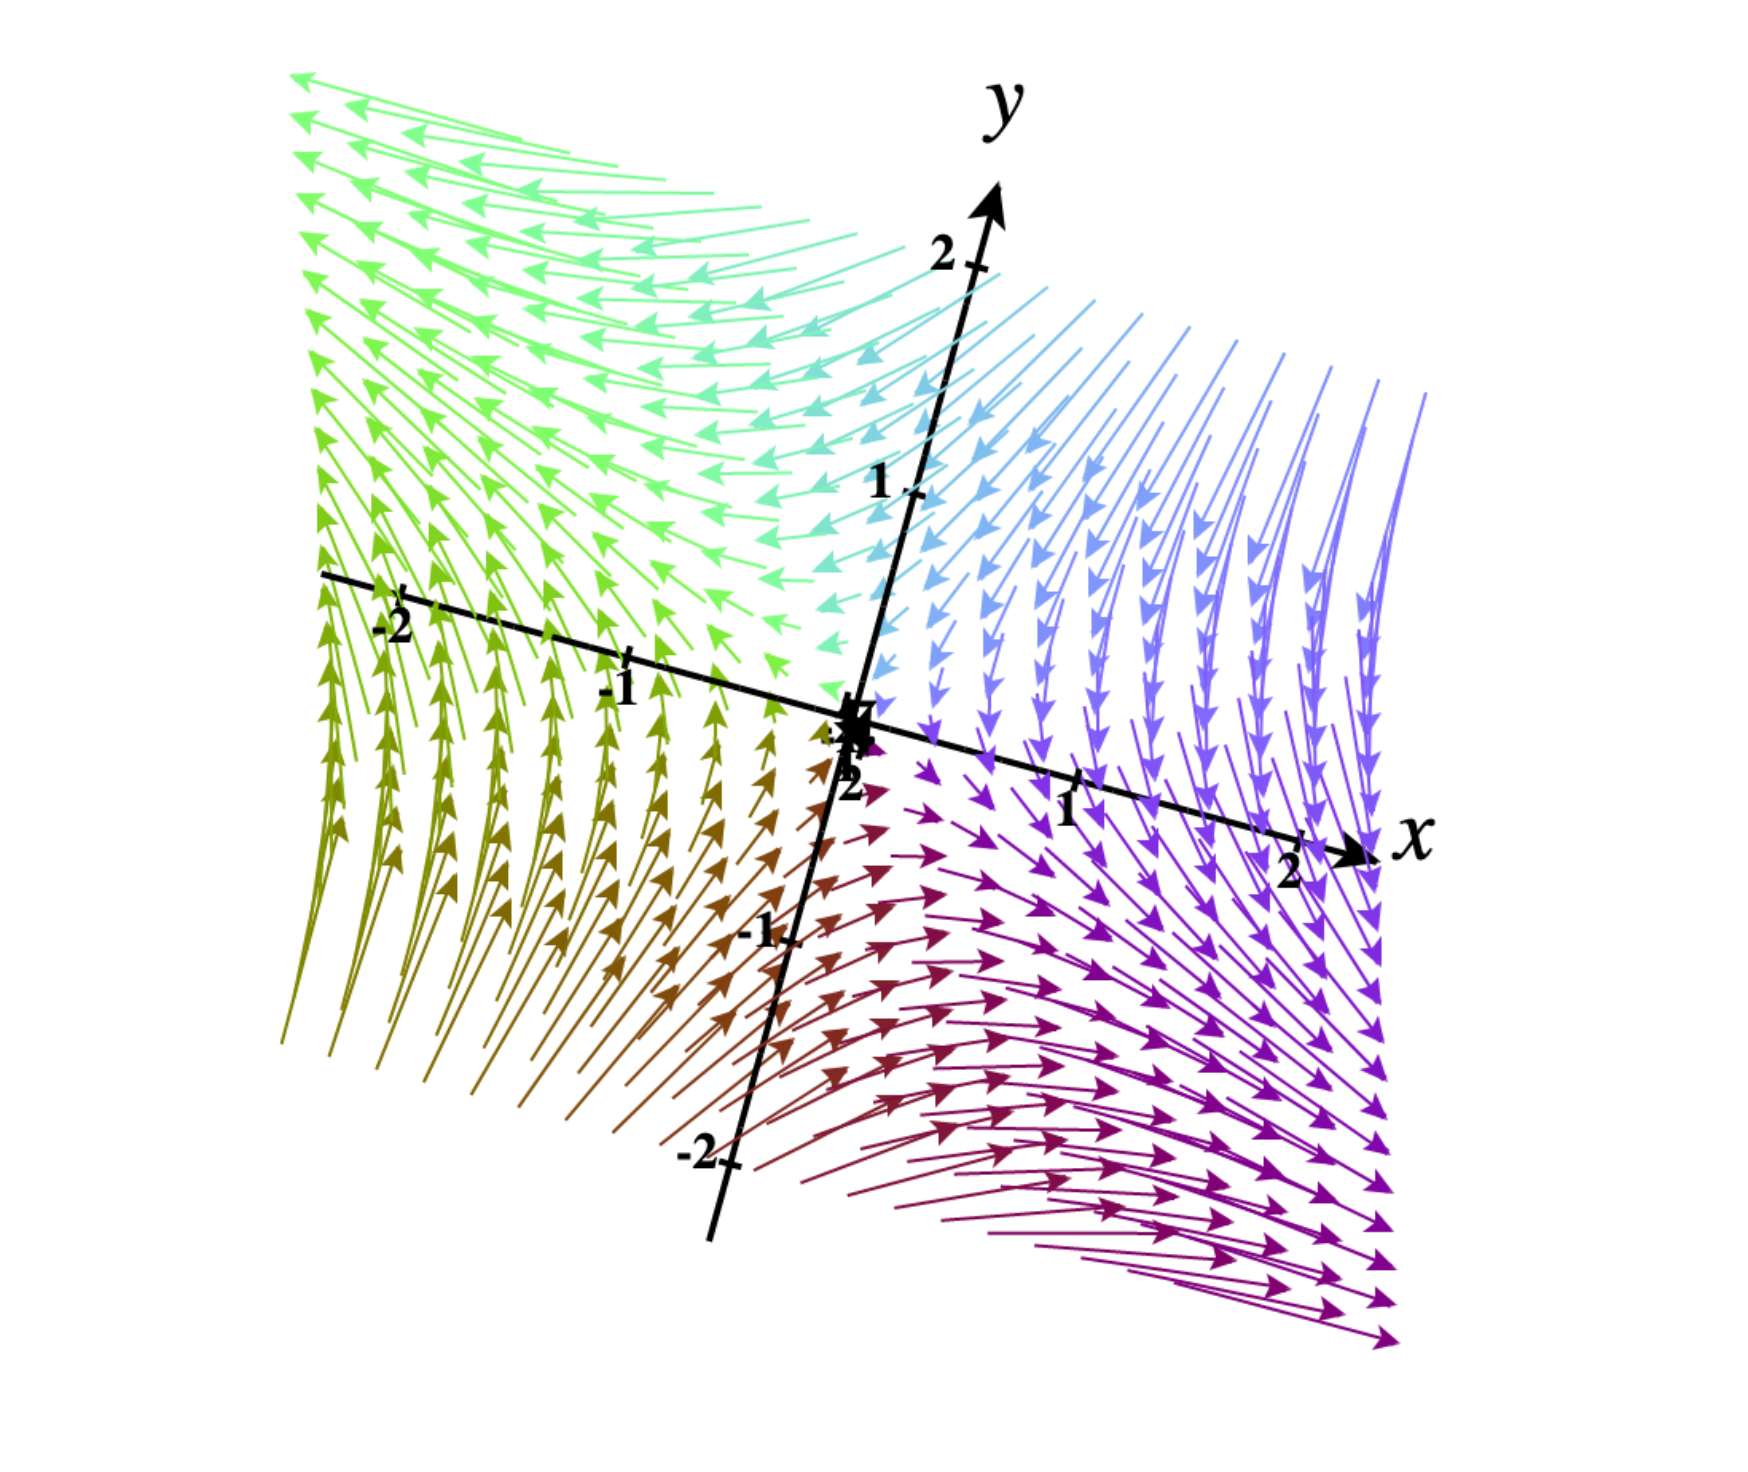
\includegraphics[width=.7\textwidth]{Images/linear_system_vfield.png}
    \end{figure}
    \item ~
    \begin{enumerate}[i.]
        \item If the starting point is $(x_0,y_0)=(0,0)$ then we have
        \begin{align*}
            x' &= 0-0 = 0\\
            y' &= -0-0=0,
        \end{align*}
        so both $x'=y'=0$. Thus, if we start at the origin, we stay at the origin.
        \item If we start at $(x_0,y_0)=(1,1)$ then we have
        \begin{align*}
            x' &= 1-1 = 0\\
            y' &= -1 -1 = -2
        \end{align*}
        so we have no initial movement in the $x$-direction and only negative movement in the $y$-direction. However, it seems over time that the $x$-values grow and the $y$-values continue to decrease.
        
        \item This point is similar the previous as we have $x' =0$ initially but $y'$ is positive instead of negative.  In this case we an see that we are carried in the negative $x$-direction and the positive $y$-direction over time.
    \end{enumerate}
\end{enumerate}
\end{solution}
\vspace*{.5cm}

\noindent\textbf{*Problem 2.} With the same linear system as in 1, do the following.
\begin{enumerate}[(a)]
    \item Compute the eigenvalues of the matrix $M$.
    \item Compute the eigenvectors of the matrix $M$.
    \item Write the general solution for this system.
    \item Find the particular solution corresponding to the initial data $(x(0),y(0))=(1,1)$.
\end{enumerate}
\begin{solution}~
\begin{enumerate}[(a)]
    \item The eigenvalues are found by solving
    \[
    \det(M-\lambda I)=0.
    \]
    So we have
    \begin{align*}
        \det(M-\lambda I)&=0\\
        \left| \begin{bmatrix} 1-\lambda & -1 \\ -1 & -1-\lambda \end{bmatrix} \right| &= 0\\
        (1-\lambda)(-1-\lambda)-1&=0\\
        -1+\lambda-\lambda + \lambda^2 -1 &=0\\
        \lambda^2 -2 &=0\\
        \lambda^2 &=2\\
        \implies \lambda &= \pm \sqrt{2}.
    \end{align*}
    We'll set $\lambda_1= \sqrt{2}$ and $\lambda_2=-\sqrt{2}$.
    \item Now, to find the eigenvectors, we want to find a vector $\mathbf{e}$ that solves
    \[
    (M-\lambda)\mathbf{e} =\mathbf{0}.
    \]
    \noindent \underline{For $\lambda_1 =\sqrt{2}$}
    We have,
    \[
    \begin{bmatrix} 1-\sqrt{2} & -1 \\ -1 & -1 -\sqrt{2} \end{bmatrix} \begin{bmatrix} e_1 \\ e_2 \end{bmatrix} = \begin{bmatrix} 0 \\ 0 \end{bmatrix}
    \]
    We can make the augmented matrix, and solve by row reduction. So we have
    \begin{align*}
    \left[
    \begin{array}{cc|c}
        1-\sqrt{2} & -1 & 0  \\
        -1 & -1 -\sqrt{2} & 0 
    \end{array}\right]
    &\underrightarrow{\textrm{Add R2 from R1}}    
    \left[
    \begin{array}{cc|c}
        -\sqrt{2} & -2-\sqrt{2} & 0  \\
        -1 & -1 -\sqrt{2} & 0 
    \end{array}\right]\\
    \underrightarrow{\textrm{Multiply R2 by $\sqrt{2}$}} 
    \left[
    \begin{array}{cc|c}
        -\sqrt{2} & -2-\sqrt{2} & 0  \\
        -\sqrt{2} & -2 -\sqrt{2} & 0 
    \end{array}\right]&\underrightarrow{\textrm{Subtract R1 from R2}}    
    \left[
    \begin{array}{cc|c}
        -\sqrt{2} & -2-\sqrt{2} & 0  \\
        0 & 0 & 0 
    \end{array}\right].
    \end{align*}
    This gives us the equation
    \begin{align*}
        -\sqrt{2}x+(-2-\sqrt{2})y&=0\\
        -\sqrt{2}x&=(2+\sqrt{2})y\\
        x&=\left(\frac{-2}{\sqrt{2}}-1\right)y\\
        x&= (-1-\sqrt{2})y.
    \end{align*}
    So choose $y=1$ and we find that the eigenvector corresponding to $\lambda_1$ is
    \[
    \mathbf{e}_1 = \begin{bmatrix} -1-\sqrt{2} \\ 1\end{bmatrix}.
    \]
    
    \noindent \underline{For $\lambda_2=-\sqrt{2}$}
    The work is very similar, and you find that the corresponding eigenvector is
    \[
    \mathbf{e}_2 = \begin{bmatrix} -1+\sqrt{2} \\ 1 \end{bmatrix}.
    \]
    \item The general solution is
    \[
    \begin{bmatrix} x(t) \\ y(t) \end{bmatrix} = c_1 e^{\sqrt{2}t} \begin{bmatrix} -1-\sqrt{2} \\ 1 \end{bmatrix} + c_2 e^{-\sqrt{2}t} \begin{bmatrix} -1 + \sqrt{2} \\ 1 \end{bmatrix}.
    \]
    \item We use the initial data so we know
    \begin{align*}
    \begin{bmatrix} x(0) \\ y(0) \end{bmatrix} = \begin{bmatrix} 0 \\ 0 \end{bmatrix} &= c_1 e^{\sqrt{2}\cdot 0} \begin{bmatrix} -1-\sqrt{2} \\ 1 \end{bmatrix} + c_2 e^{-\sqrt{2}\cdot 0} \begin{bmatrix} -1 + \sqrt{2} \\ 1 \end{bmatrix}\\
    &= \begin{bmatrix} c_1(-1-\sqrt{2}) \\ c_1 \end{bmatrix} + \begin{bmatrix} c_2 (-1+\sqrt{2})\\ c_2 \end{bmatrix}.
    \end{align*}
    This gives us the following system of equations
    \begin{align}
        1 &= c_1(-1-\sqrt{2})+c_2(-1+\sqrt{2})\\
        1 &= c_1 + c_2.
    \end{align}
    Note that (2) gives us that $c_2=1-c_1$ and we plug this into (1) to find
    \begin{align*}
    1 &= c_1(-1-\sqrt{2})+(1-c_1)(-1+\sqrt{2})\\
    1 &= -c_1 -\sqrt{2}c_1 -1 +\sqrt{2}+c_1-\sqrt{2}c_1\\
    2-\sqrt{2} &= -2\sqrt{2}c_1\\
    \implies c_1 &= \frac{1}{2}-\frac{1}{\sqrt{2}}.
    \end{align*}
    Thus, $c_2 = \frac{1}{2}+\frac{1}{\sqrt{2}}$. So the particular solution is
    \[
    \begin{bmatrix} x_p(t) \\ y_p(t) \end{bmatrix} = \left(\frac{1}{2}-\frac{1}{\sqrt{2}}\right) e^{\sqrt{2}t} \begin{bmatrix} -1-\sqrt{2} \\ 1 \end{bmatrix} + \left( \frac{1}{2}+\frac{1}{\sqrt{2}}\right) e^{-\sqrt{2}t} \begin{bmatrix} -1 + \sqrt{2} \\ 1 \end{bmatrix}
    \]
\end{enumerate}
\end{solution}

\vspace*{.5cm}

\noindent\textbf{Problem 3.} Solving the one dimensional Laplace equation is much like an ODE.  However, the data given looks a bit different.  So consider the following set up.

Consider the Laplace equation
\[
\Delta u(x) = \frac{d^2u}{dx^2} = 0
\]
on the interval $\Omega = (0,1)$ with boundary conditions $u(0)=0$ and $u(1)=1$.  
\begin{enumerate}[(a)]
    \item This equation is separable. To find $u$, take two antiderivatives of
    \[
    \frac{d^2u}{dx^2}=0.
    \]
    \item To verify you did this correctly, take two derivatives of your function to see that you get $0$.
    \item Your function should have two undetermined constants.  Solve for these constants using the boundary conditions provided.
\end{enumerate}
\begin{solution}~
\begin{enumerate}[(a)]
    \item We take an antiderivative
    \begin{align*}
    \int \frac{d^2u}{dx^2} dx &= \int 0 dx\\
    \frac{du}{dx} &= c_1,
    \end{align*}
    by the fundamental theorem of calculus. We can do this again and get
    \begin{align*}
    \int \frac{du}{dx}dx &= \int c_1 dx\\
    u(x) &= c_1x+c_2.
    \end{align*}
    \item We check this by taking two derivatives
    \[
    \frac{d}{dx} \frac{d}{dx} (c_1+x+c_2) = \frac{d}{dx} c_1 = 0.
    \]
    So this function does work.
    \item We know that 
    \[
    u(0)= 0=c_1(0)+c_2 
    \]
    which means $c_2=0$. Then we also have
    \[
    u(1)= 1 = c_1(1)
    \]
    which means that $c_1=1$. So we have
    \[
    u(x)=x.
    \]
\end{enumerate}
\end{solution}
\vspace*{.5cm}

\noindent\textbf{Problem 4.} The methods for solving many PDEs are beyond the scope of this class, but we can still see what solutions behave like and a bit of how to find these. What we'll do below are a few steps of the method of \emph{separation of variables} (not to be confused with separable ODE!) 

Consider the heat equation in one dimension on the region $\Omega = (0,1)$
\[
\frac{\partial u}{\partial t}(x,t) - \frac{\partial^2 u}{\partial x^2}(x,t) = 0
\]
with boundary conditions $u(0,t)=0$ and $u(1,t)=0$, and initial condition $u(x,0)=\sin(\pi x)$.
\begin{enumerate}[(a)]
    \item Show that $f(x)=\sin(\pi x)$ is a solution to
    \[
    f''(x)=-\pi^2 f(x)
    \]
    with $f(0)=0$ and $f(1)=0$.
    \item Show that $g(t) = e^{-\pi^2 t}$ is a solution to 
    \[
    g'(t) = -\pi^2 g(t)
    \]
    with $g(0)=1$.
    \item Show that $u(x,t)=f(x)g(t)$ solves the heat equation with these boundary and initial conditions.
\end{enumerate}

\begin{solution}~
\begin{enumerate}[(a)]
    \item We have
    \begin{align*}
    \frac{d^2f}{dx^2}&= \frac{d}{dx}\frac{d}{dx} \sin(\pi x)\\
    &= \pi \frac{d}{dx} \cos(\pi x)\\
    &= -\pi^2 \sin(\pi x)\\
    &= -\pi^2 f(x).
    \end{align*}
    So we have the ODE is solved.  Then we also check
    \[
    f(0)=\sin(\pi 0) = 0
    \]
    and
    \[
    f(1)=\sin(\pi) = 0
    \]
    and so the boundary conditions are satisfied.
    \item We have
    \begin{align*}
        \frac{dg}{dt} = \frac{d}{dt} e^{-\pi^2 t} = -\pi^2 e^{-\pi^2 t} = -\pi^2 g(t).
    \end{align*}
    Then note that
    \[
    g(0) = e^{-\pi^2 \cdot 0} = 1.
    \]
    So this solves the PDE and initial value.
    
    \item We have
    \begin{align*}
        \frac{\partial}{\partial t} f(x)g(t) - \frac{\partial^2}{\partial x^2} f(x)g(t) &= f(x) g'(t)-f''(x)g(t)\\
        &= -\pi^2 f(x)g(t)+\pi^2 f(x)g(t)\\
        &= 0.
    \end{align*}
    So indeed this function $u(x,t)$ does satisfy the PDE.  Now we also check
    \[
    u(0,t) = e^{-\pi^2\cdot 0} \sin(0)=0
    \]
    and
    \[
    u(1,1) = e^{-\pi^2} \sin(\pi)=0,
    \]
    so the boundary conditions are satisfied. Lastly, we have
    \[
    u(x,0)=e^{-\pi^2 \cdot 0 }\sin(\pi x) = \sin(\pi x),
    \]
    so the initial conditions are satisfied.
\end{enumerate}
\end{solution}
\vspace*{.5cm}

\noindent\textbf{Problem 5.} With our solution from 4, we can analyze the behavior of the system.  The physical phenomenon that Problem 4 modelled was a thin rod (the segment $(0,1)$) that had an initial temperature distribution $\sin(\pi x)$, i.e. it was warmer in the middle and coldest on the ends.  The boundary conditions $u(0)=0$ and $u(1)=0$ can be thought of as attaching a thermocouple at each end that holds the end temperature at $0$ degrees.  
\begin{enumerate}[(a)]
    \item Plot the function on CalcPlot3D by plotting
    \[
    z=e^{-\pi^2 y} \sin(\pi x)= u(x,y),
    \]
    where we just let the $t$ variable be denoted by $y$ to plot this function.
    \item Can you explain what happens as time $t$ moves forward based on your intuition, plot, or by the equation we found in 4?
\end{enumerate}

\begin{solution}
\begin{enumerate}[(a)]
    \item Here is the plot.
    \begin{figure}[H]
        \centering
        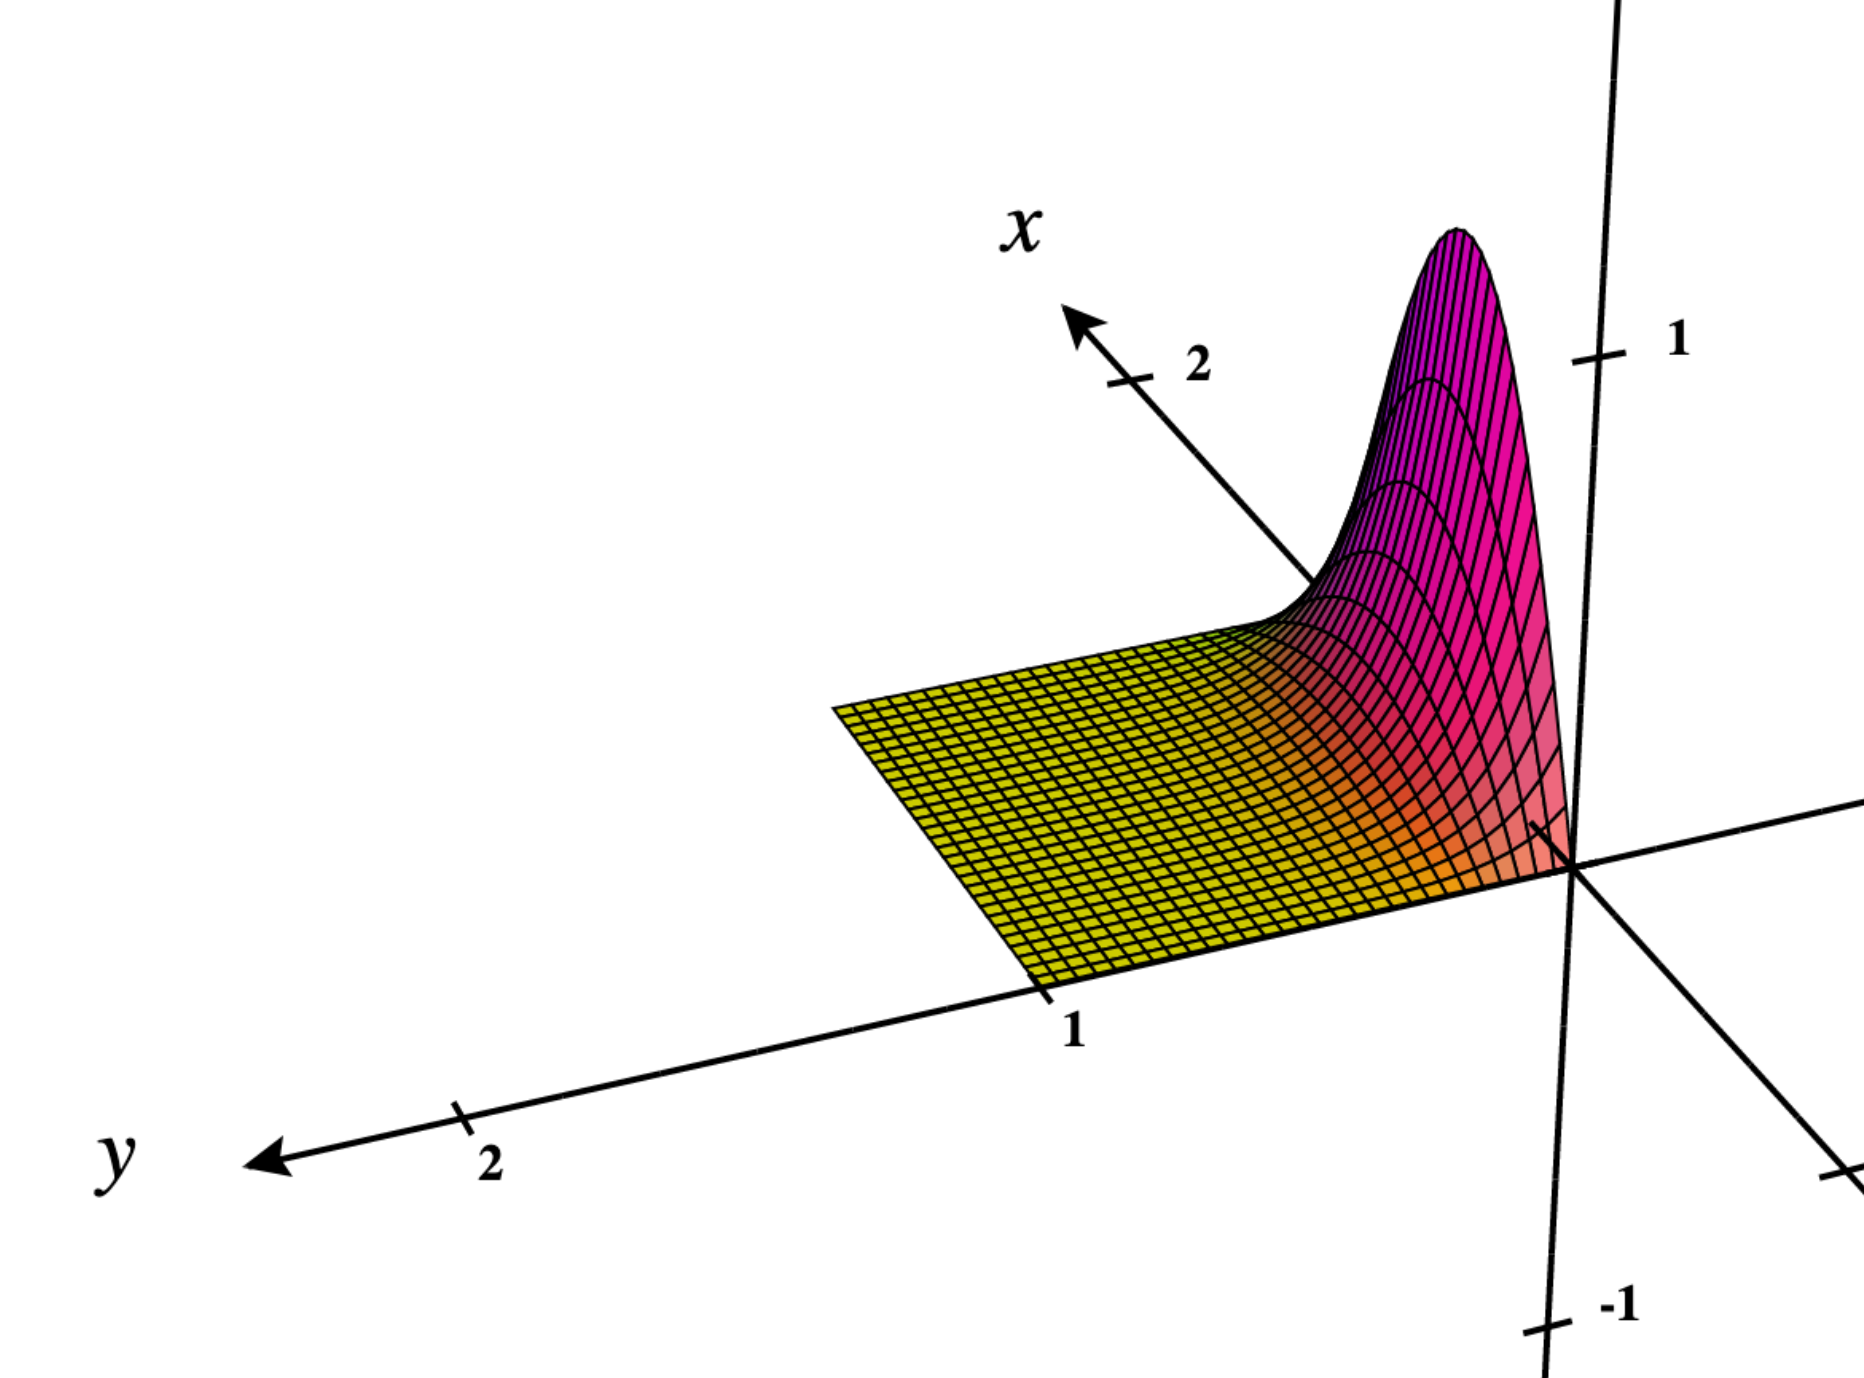
\includegraphics[width=.7\textwidth]{Images/heat_equation_solution.png}
    \end{figure}
    \item As $t$ increases, the temperature starts to regularize in the rod.  We can see that as $t$ gets very large, we expect the temperature in the whole rod to be $0$.  This is fairly intuitive.  If we old the ends of a rod at some temeprature, we do expect the temeprature to equalize throughout the rod given enough time.
    
    Using the solution equation, we can just see that $e^{-\pi^2 t}$ gets smaller and smaller as $t$ increases.
\end{enumerate}

\end{solution}


\end{document}  